\documentclass[border=3pt]{standalone}
\usepackage{fontspec}
\newfontfamily\chessfont{Apple Symbols}
\usepackage{tikz}
\usepackage{pgfplots}
\pgfplotsset{compat=1.17}
\definecolor{light}{HTML}{EDEDED}
\definecolor{dark}{HTML}{7389B8}
\definecolor{edge}{HTML}{4A4A4A}
\definecolor{blue2}{HTML}{B9C6E0}
\begin{document}
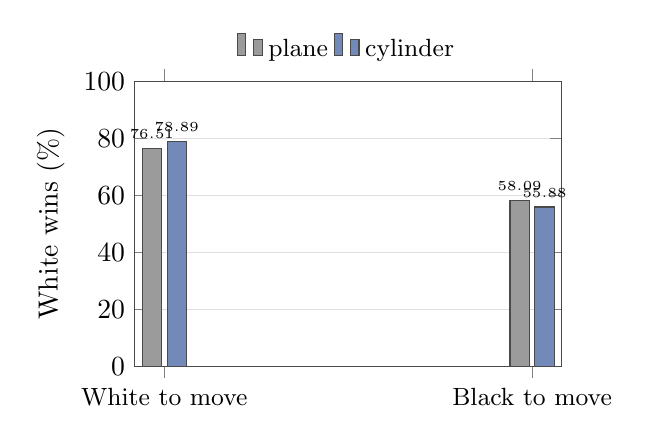
\begin{tikzpicture}\begin{axis}[ybar, bar width=7pt, width=7cm, height=5.2cm,
  ymin=0, ymax=100, ylabel={White wins (\%)}, symbolic x coords={White to move,Black to move}, xtick=data,
  x tick label style={font=\small}, ymajorgrids, grid style={gray!25}, enlarge x limits=0.08,
  legend style={at={(0.5,1.03)}, anchor=south, legend columns=2, draw=none, font=\small},
  axis line style={edge}, nodes near coords, nodes near coords style={font=\tiny}]
\addplot[fill=edge!55, draw=edge] coordinates {(White to move,76.51) (Black to move,58.09)};
\addlegendentry{plane}
\addplot[fill=dark, draw=edge] coordinates {(White to move,78.89) (Black to move,55.88)};
\addlegendentry{cylinder}
\end{axis}\end{tikzpicture}
\end{document}
